\chapter{System architecture}

\section{Hardware architecture}
\subsection{Overview}
%intro

Choosing the right components is essential for keeping cost low and meeting the requirements for the system.

%controller

%gps

\subsubsection{General BDD}
\begin{figure}[H]
	\centering
	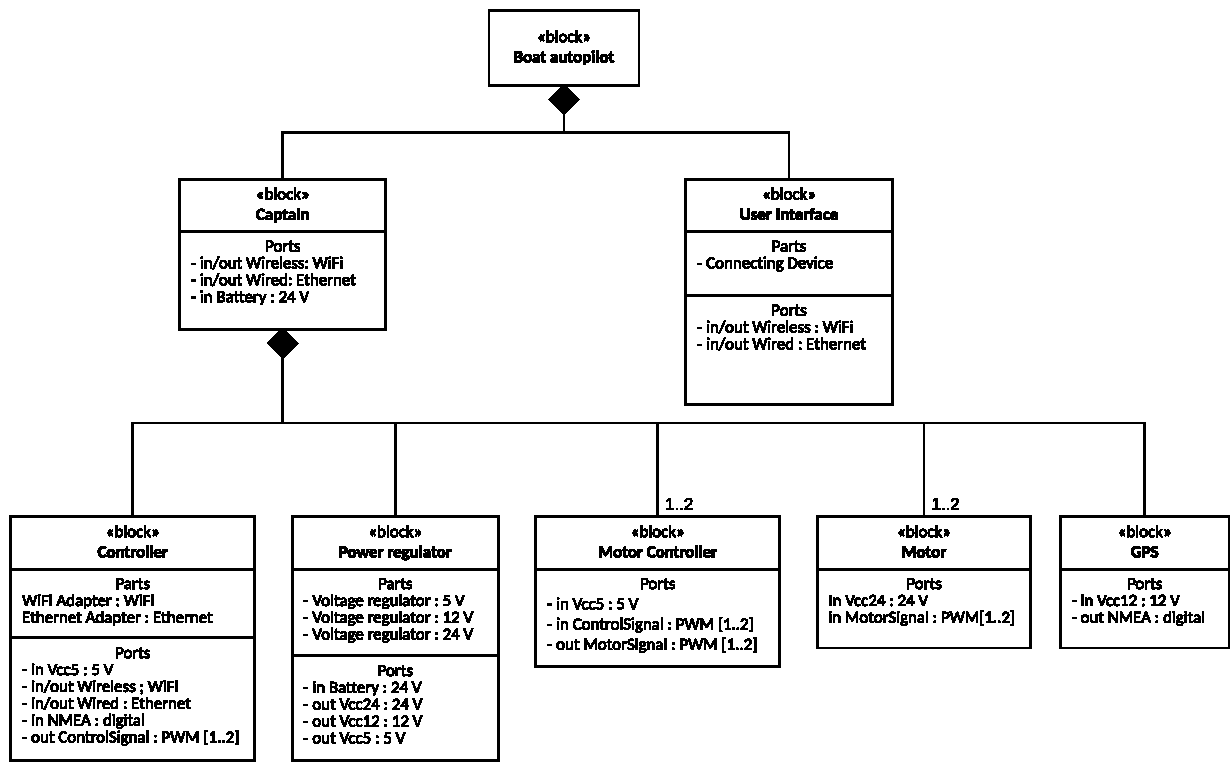
\includegraphics[width=1\linewidth]{Images/System_architecture/General_BDD}
	\caption{General BDD}
\end{figure}

k

\subsubsection{General IBD}
\begin{figure}[H]
	\centering
	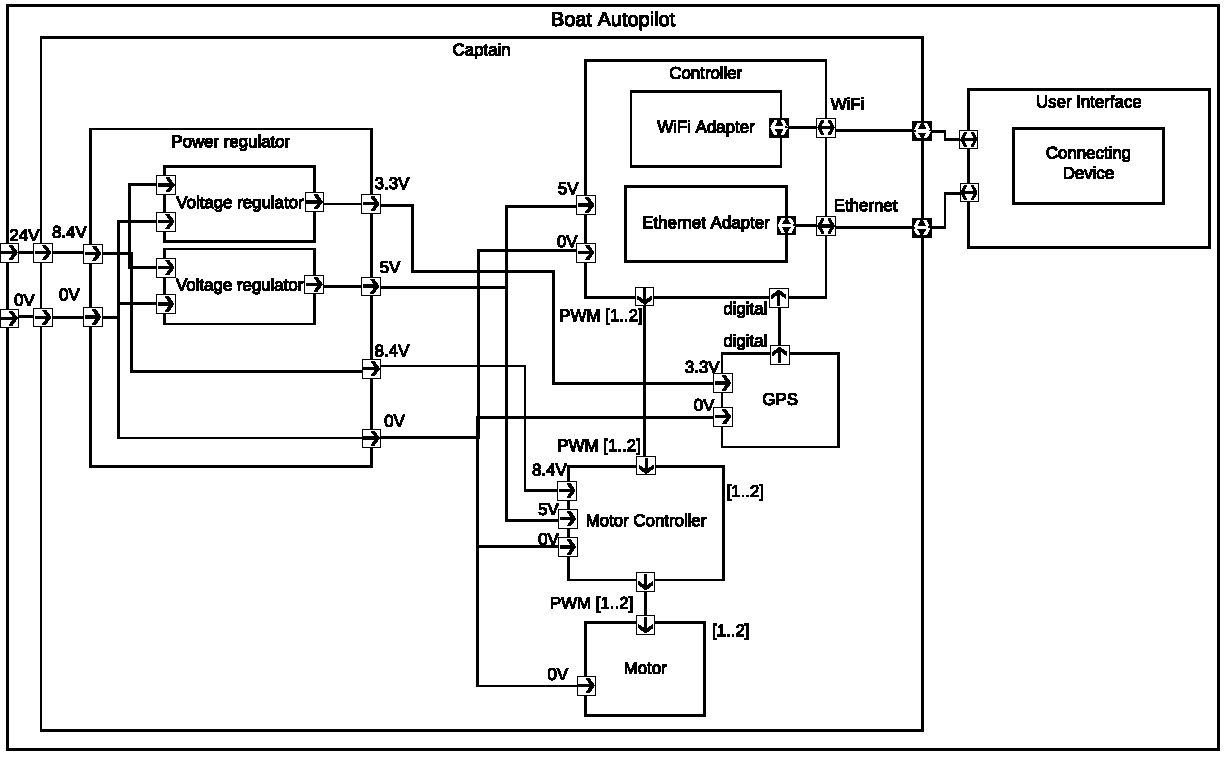
\includegraphics[width=1\linewidth]{Images/System_architecture/General_IBD}
	\caption{General IBD}
\end{figure}

k

\subsubsection{Signal list}

%TODO change ibd so every signal has a name
Table~\ref*{table: General IBD} shows the signal list for the general system.
\begin{table}[htbp]
	\centering
	\begin{tabular}{|l|l|l|}
		\hline
		\textbf{Signal type} 	&\textbf{Name}		&\textbf{Description} \\\hline
		8.4V			&Vsupply	&8.4V supply to Power regulator from battery\\\hline
		
		8.4V			&Vcc8		&8.4V supply to Motor Controller\\\hline
		5V			&Vcc5		&5V supply to Controller and Motor Controller\\\hline
		3.3V			&Vcc3		&3.3V supply to GPS\\\hline
		0V			&0V			&System ground\\\hline
		PWM	&MotConPWM	&PWM-signal to Motor Control, 5V\\\hline
		PWM	&MotorPWM	&PWM-signal to Motor, 8.4V\\\hline
		UART		&GPS		&GPS data to Controller through UART\\\hline	
		WiFi		&WiFi		&WiFi signal between Controller and User interface\\\hline
		Ethernet	&Ethernet	&Ethernet signal between Controller and User interface\\\hline
		
		
	\end{tabular}
	\caption{Signal list for General IBD}
	\label{table: General IBD}
\end{table}

\section{Software architecture}
k

\begin{figure}[H]
	\centering
	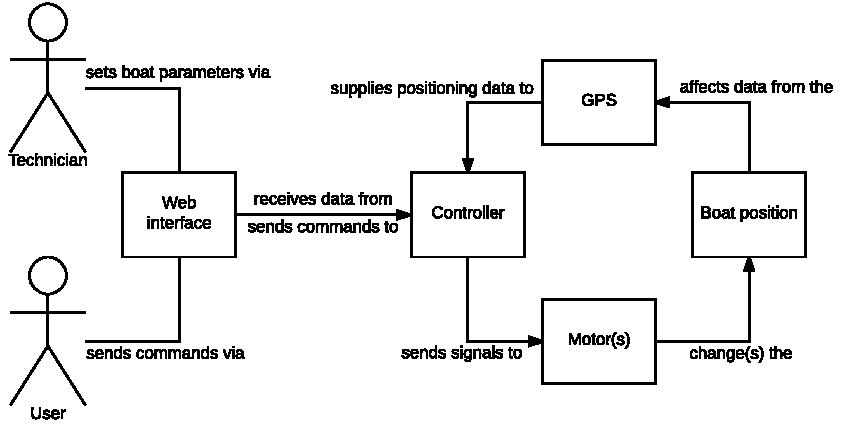
\includegraphics[width=1\linewidth]{Images/System_architecture/Domain_Model}
	\caption{Domain Model}
\end{figure}

k

\begin{figure}[H]
	\centering
	\includegraphics[width=1\linewidth]{Images/System_architecture/Application_Model}
	\caption{Application Model}
\end{figure}

k

\begin{figure}[H]
	\centering
	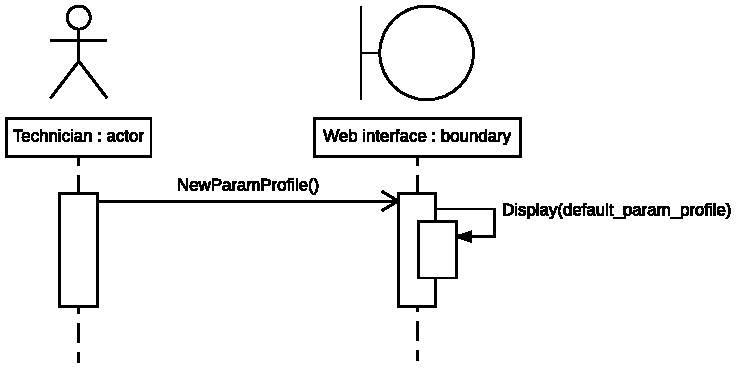
\includegraphics[width=1\linewidth]{Images/System_architecture/Use_case_1_SD}
	\caption{Sequence diagram for Use case 1 - New parameter profile}
\end{figure}

k

\begin{figure}[H]
	\centering
	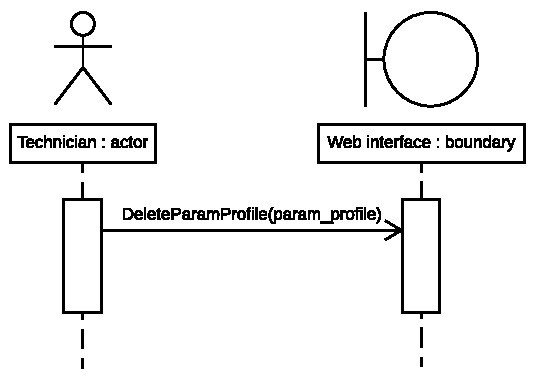
\includegraphics[width=1\linewidth]{Images/System_architecture/Use_case_2_SD}
	\caption{Sequence diagram for Use case 2 - Delete parameter profile}
\end{figure}

k

\begin{figure}[H]
	\centering
	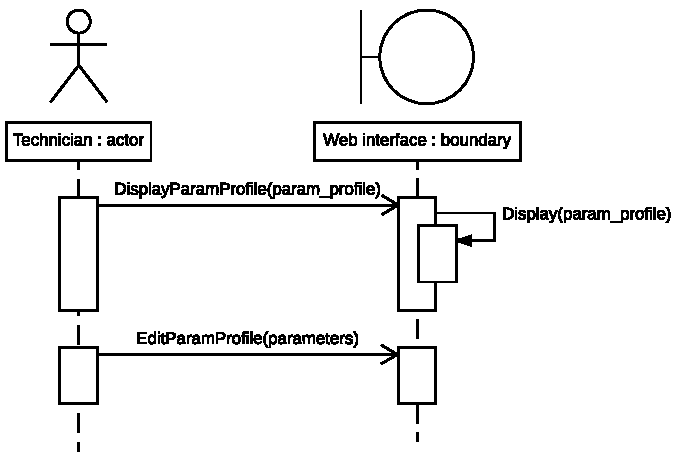
\includegraphics[width=1\linewidth]{Images/System_architecture/Use_case_3_SD}
	\caption{Sequence diagram for Use case 3 - Edit parameter profile}
\end{figure}

k

\begin{figure}[H]
	\centering
	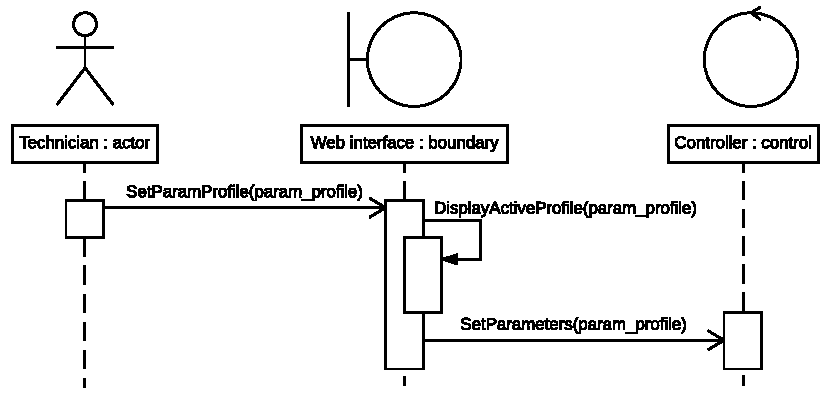
\includegraphics[width=1\linewidth]{Images/System_architecture/Use_case_4_SD}
	\caption{Sequence diagram for Use case 4 - Set active parameter profile}
\end{figure}

k

\begin{figure}[H]
	\centering
	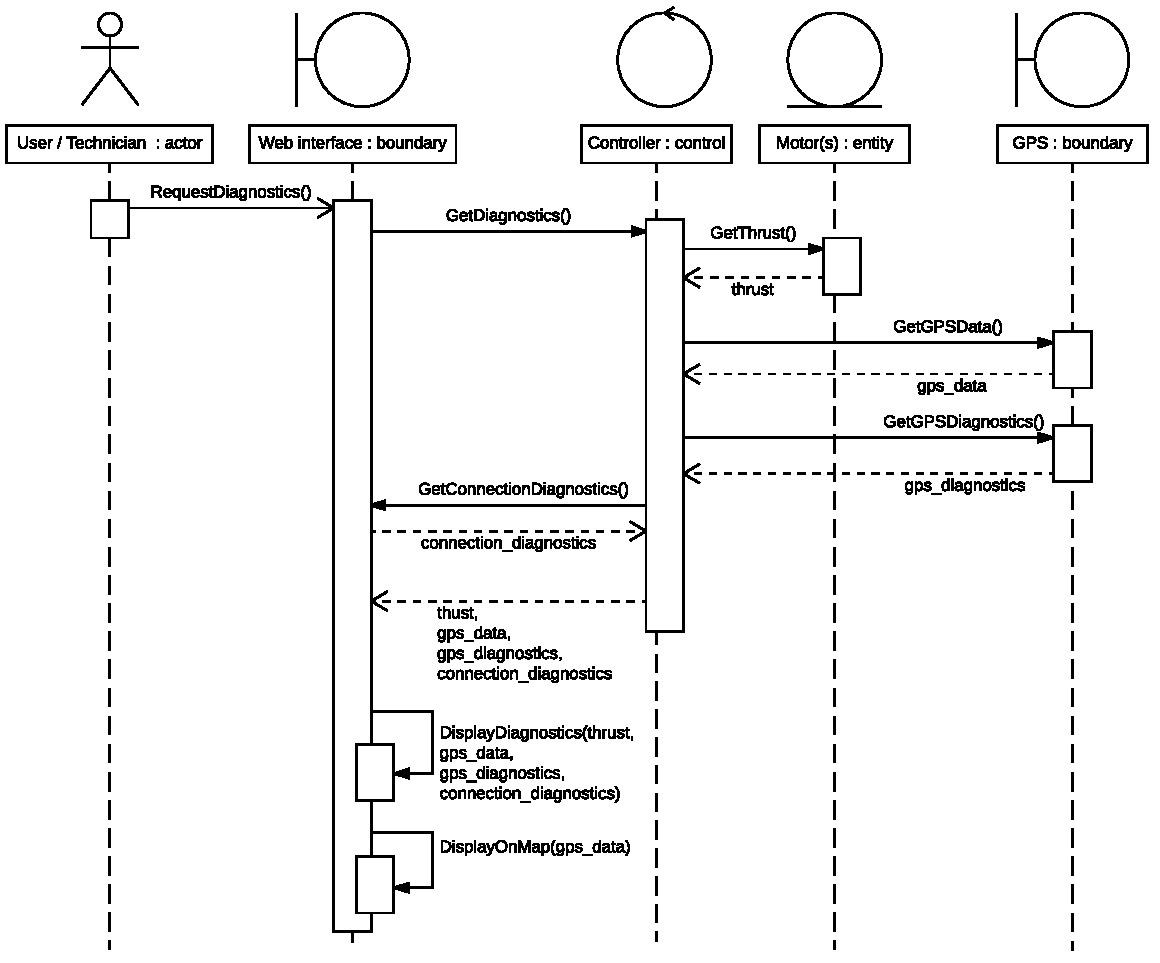
\includegraphics[width=1\linewidth]{Images/System_architecture/Use_case_5_SD}
	\caption{Sequence diagram for Use case 5 - Request diagnostics}
\end{figure}

k

\begin{figure}[H]
	\centering
	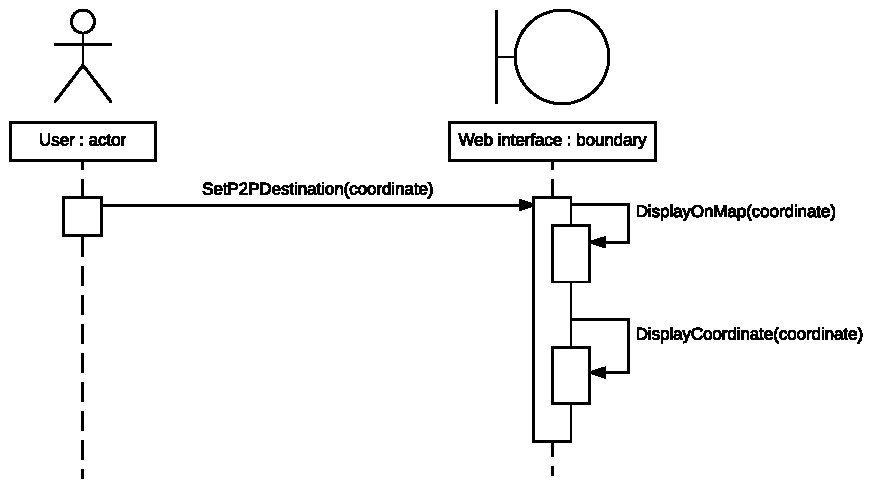
\includegraphics[width=1\linewidth]{Images/System_architecture/Use_case_6_SD}
	\caption{Sequence diagram for Use case 6 - Set point to point destination}
\end{figure}

k

\begin{figure}[H]
	\centering
	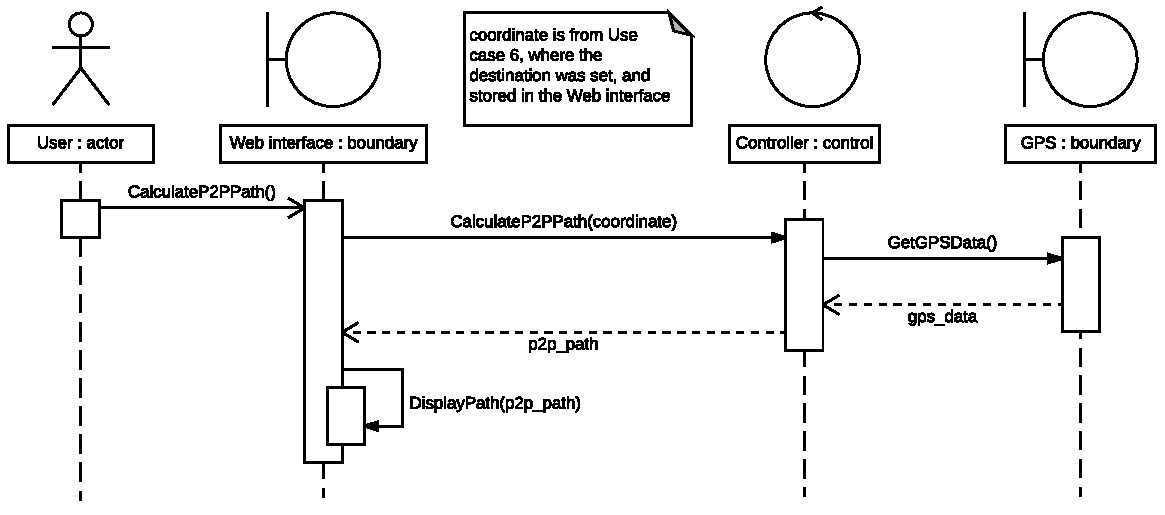
\includegraphics[width=1\linewidth]{Images/System_architecture/Use_case_7_SD}
	\caption{Sequence diagram for Use case 7 - Calculate point to point path}
\end{figure}

k

\begin{figure}[H]
	\centering
	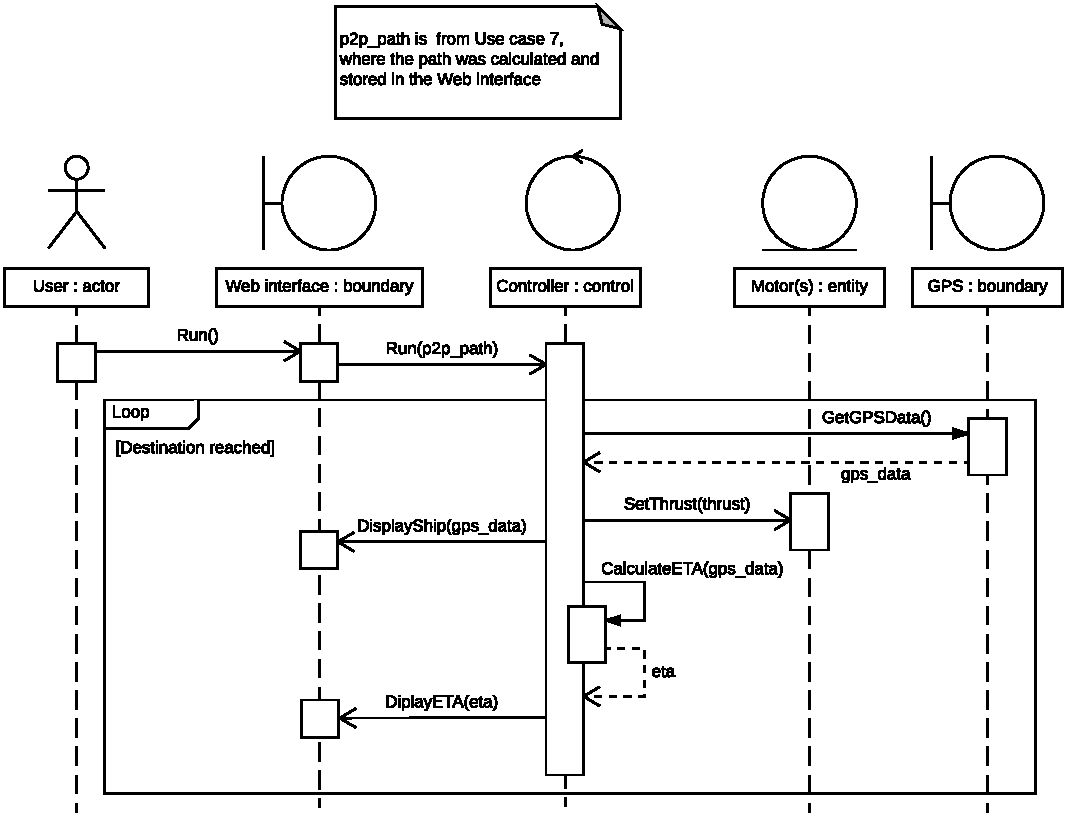
\includegraphics[width=1\linewidth]{Images/System_architecture/Use_case_8_SD}
	\caption{Sequence diagram for Use case 8 - Run point to point path}
\end{figure}

k

\begin{figure}[H]
	\centering
	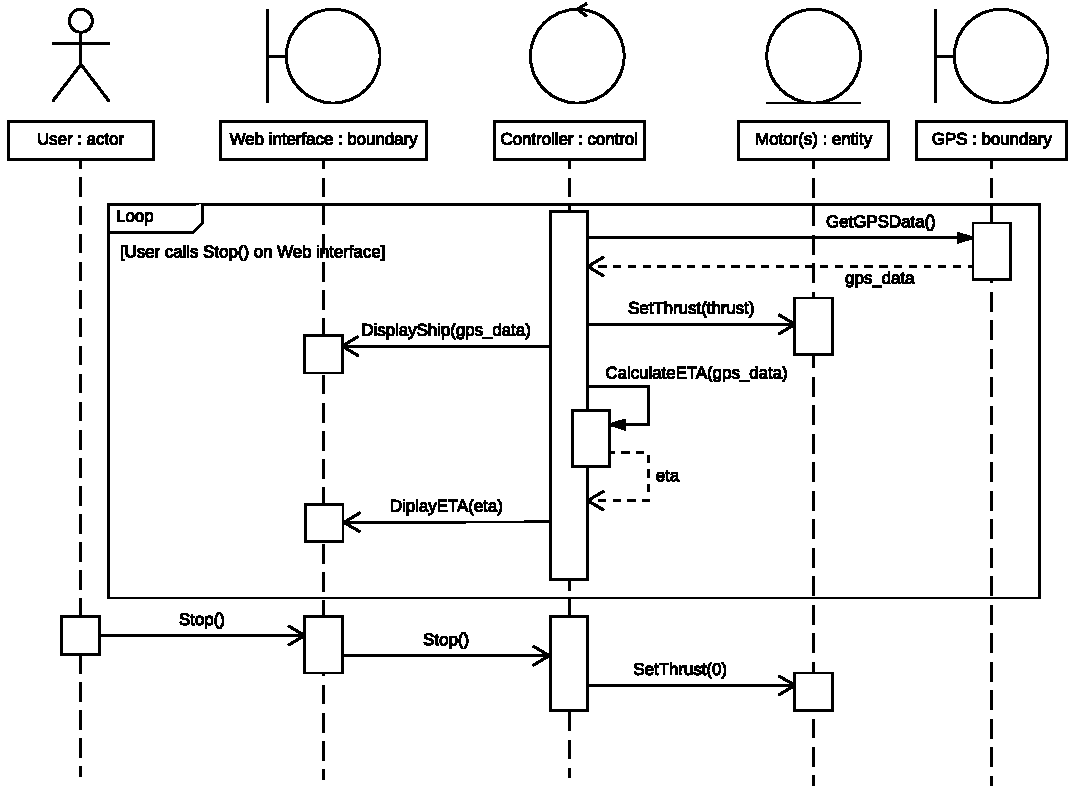
\includegraphics[width=1\linewidth]{Images/System_architecture/Use_case_9_SD}
	\caption{Sequence diagram for Use case 9 - Stop point to point path}
\end{figure}

k

\begin{figure}[H]
	\centering
	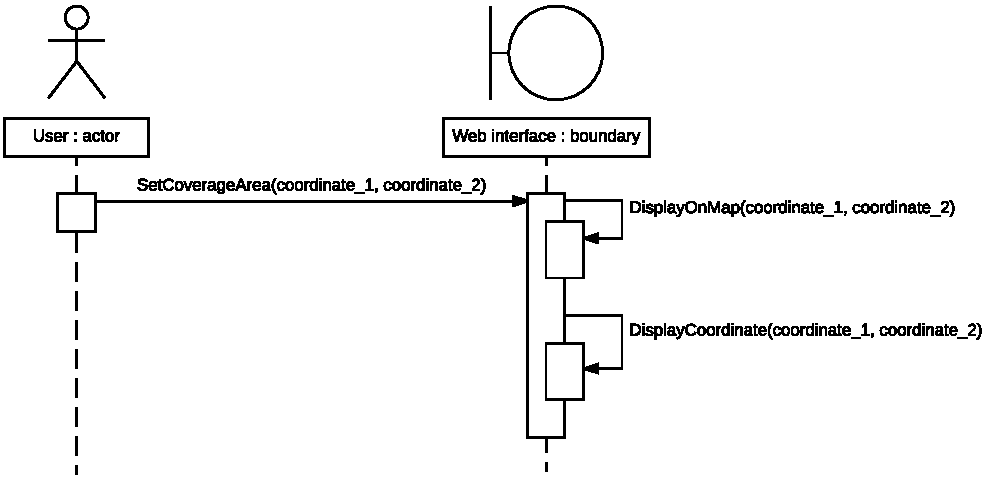
\includegraphics[width=1\linewidth]{Images/System_architecture/Use_case_10_SD}
	\caption{Sequence diagram for Use case 10 - Set coverage area}
\end{figure}

k

\begin{figure}[H]
	\centering
	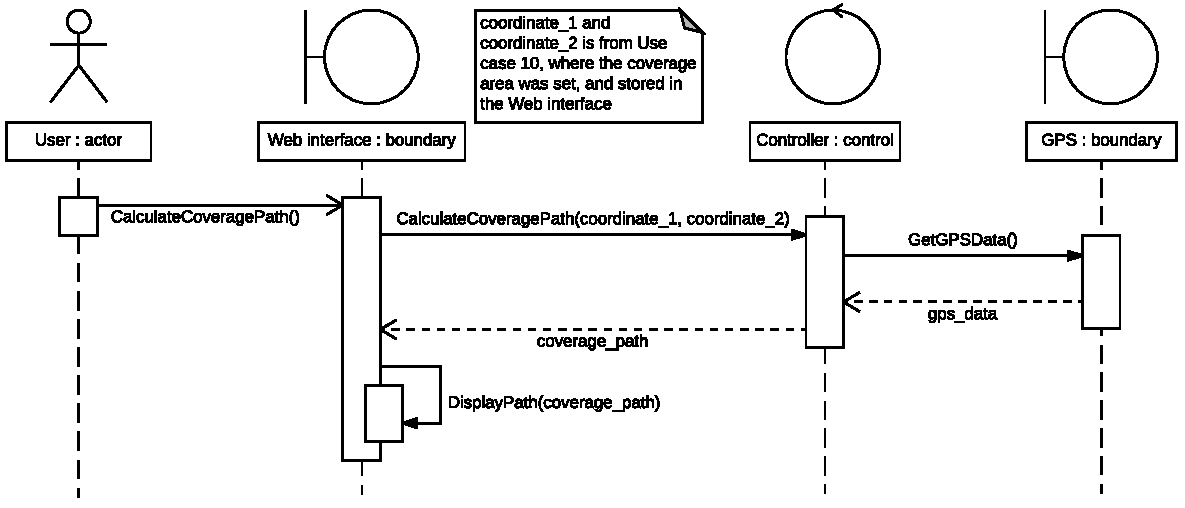
\includegraphics[width=1\linewidth]{Images/System_architecture/Use_case_11_SD}
	\caption{Sequence diagram for Use case 11 - Calculate coverage path}
\end{figure}

k

\begin{figure}[H]
	\centering
	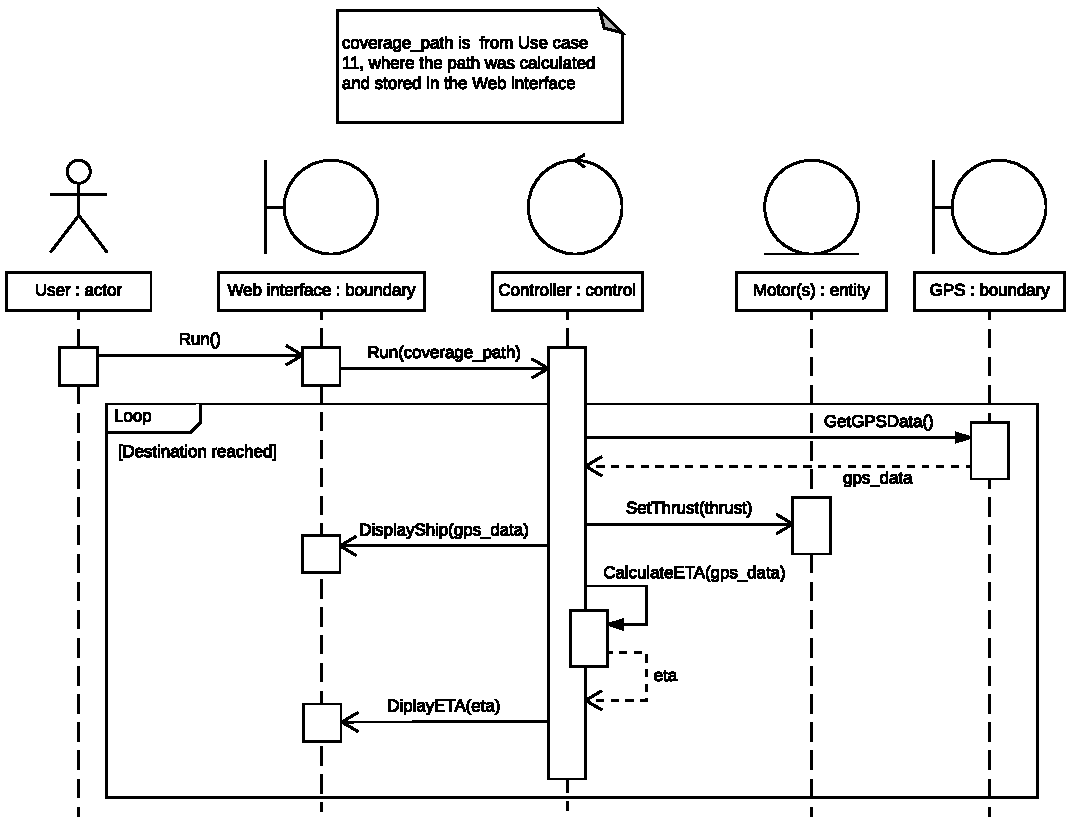
\includegraphics[width=1\linewidth]{Images/System_architecture/Use_case_12_SD}
	\caption{Sequence diagram for Use case 12 - Run coverage path}
\end{figure}

k

\begin{figure}[H]
	\centering
	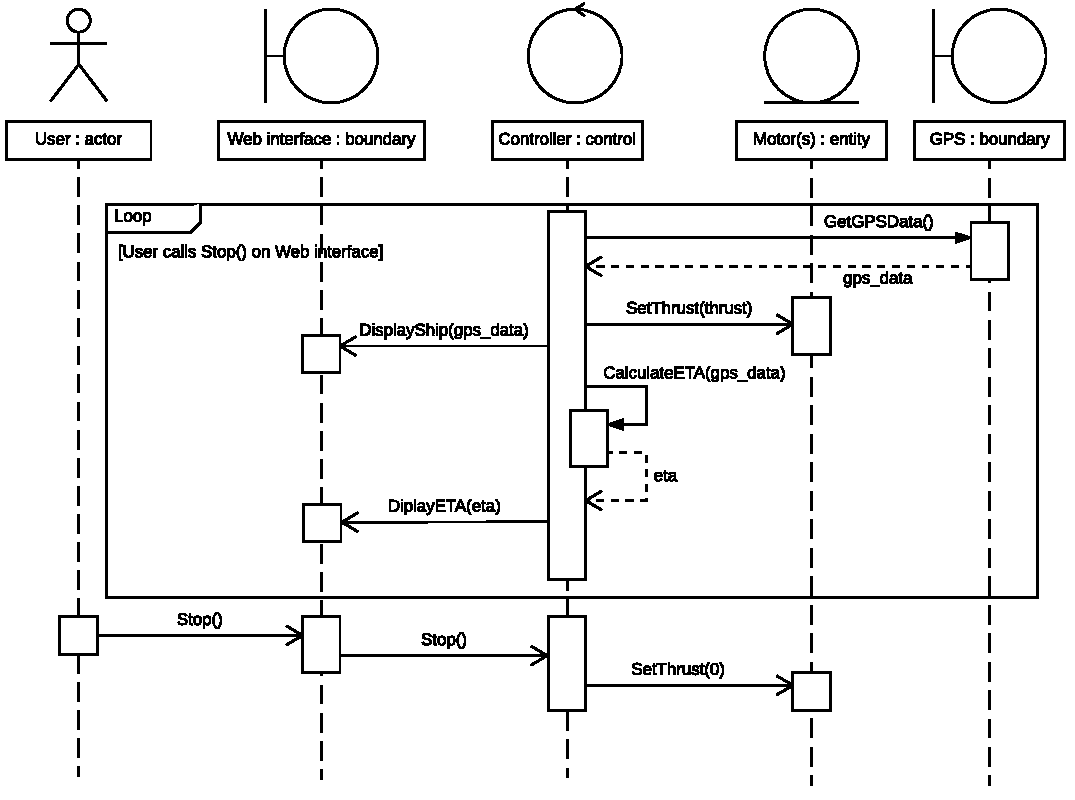
\includegraphics[width=1\linewidth]{Images/System_architecture/Use_case_13_SD}
	\caption{Sequence diagram for Use case 13 - Stop coverage path}
\end{figure}

k

